\chapter{Infrastruktura i proces wdrożeniowy}

\section{Stack technologiczny}
\par
System opiera się na skonteneryzowanych aplikacjach komunikujących się ze sobą w architekturze \gls{N-Tier} z wykorzystaniem narzędzi \gls{Docker} oraz \gls{Docker Compose}.
Wykorzystanie \gls{skrypt}ów w języku Bash ułatwia development oraz budowanie aplikacji przez osoby bez doświadczenia z \gls{Docker}em bez instalacji żadnego dodatkowego oprogramowania.
Praca przy projekcie zarządzana jest na systemie kontroli wersji \gls{Git} wraz z \gls{repozytorium} na \gls{GitHub} i testowaniu rozwiązań przy pomocy \gls{GitHub Actions}.
\par
Wybór technologii był podyktowany standardami branży oraz chęcią zespołu na zastosowanie nowoczesnych technologii.
\par
System kontroli wersji \gls{Git} jest najpopularniejszym rozwiązaniem na rynku wykorzystywanym do tworzenia oprogramowania.
Oprócz kierowania się standardami branży było to narzędzie znane każdemu z członków zespołu.
Dodatkowo \gls{Git} umożliwia nam podpięcie \gls{repozytorium} do \gls{GitHub}a.
\par
\gls{GitHub} oferuje wiele opcji, pozwala na m.in. ograniczenie dostępu do \gls{repozytorium}, ustawianie roli użytkowników, tworzenie \gls{Pull Request}ów, ustalanie reguł kiedy kod może zostać \gls{merge}'owany lub testowanie kodu za pośrednictwem \gls{GitHub Actions}.
\par
Kolejnym aspektem popierającym wykorzystywanie \gls{GitHub} jest ich wewnętrzne narzędzie \gls{GitHub Actions}.
Pozwala na testowanie naszej aplikacji za pośrednictwem \gls{runner}ów, na których wykonywane są zdefiniowane przez nas \gls{workflow}'y (\gls{CI/CD}).
Ustawienie i integrowanie tego narzędzia, zwłaszcza przy małych projektach, nie wymaga wielkiego natłoku pracy, a ewentualne zmiany lub dodawanie nowych testów jest intuicyjne.
\par
Sama aplikacja działa opierając się o \gls{Docker} i \gls{Docker Compose} - narzędzia służące do \gls{kontener}yzacji.
Rozwiązuje to problem izolacji i kompatybilności na różnych dystrybucjach, a przygotowanie środowiska do wytwarzania oprogramowania jest proste - wystarczy mieć zainstalowanego \gls{Docker}a.
\gls{Docker Compose} umożliwia na stworzenie grupy \gls{kontener}ów współpracujących ze sobą.
Ułatwia to przebudowywanie aplikacji i konfigurację konkretnych \gls{kontener}ów za pomocą \gls{manifest}u.
Aplikacja jest opakowana w \gls{skrypt}y ułatwiające budowanie, usuwanie, aktualizowanie, przebudowywanie aplikacji oraz uruchomienie jej w wersji deweloperskiej.
Zostały one stworzone głównie z myślą o członkach zespołu, którzy nie mają zbyt dużego doświadczenia w pracy z \gls{Docker}em aby ułatwić im wdrożenie w tę technologię.

\section{Repozytoria i ich zarządzanie}
\par
Na platformie \gls{GitHub} powstała organizacja pod nazwą \gls{Labbyn}.
Jej celem było przechowywanie \glslink{repozytorium}{repozytoriów} dedykowanych do naszej pracy inżynierskiej.
W pracy wykorzystane zostały dwa repozytoria:
\subsection{Repozytorium Labbyn}
\par
Główne \gls{repozytorium}, w którym przechowywany był kod źródłowy aplikacji.
\subsubsection{Struktura projektu}
\par
Każdy \gls{kontener} wymagający konfiguracji i/lub zaprogramowania posiadał swój własny dedykowany katalog.
Katalog pomocniczy "scripts" zawiera skrypty do budowania aplikacji oraz uruchamiania testowych maszyn wirtualnych.
\par
\Gls{repozytorium} ma w sobie również:
\begin{itemize}
    \item .env - katalog zawierający pliki ze zmiennymi środowiskowymi.
    W wielu przypadkach wrzucanie plików ze zmiennymi bezpośrednio w \gls{repozytorium} nie jest dobrą praktyką - może to np. prowadzić do włamań, gdy trzymane są tam hasła.
    Jednak w naszym przypadku tworzymy rozwiązanie \gls{open-source} i zachęcamy użytkowników do zmiany podanych tam wartości albo wykorzystanie innych technik do przekazania wrażliwych informacji.
    \item .gitignore oraz .gitattributes - pliki konfiguracyjne dla \gls{Git}'a
    \item docker-compose.yaml i docker-compose-dev.yaml - \gls{manifest}y \gls{Docker}owe budujące aplikacje
    \item README.md - instrukcja/opis projektu
    \item .github - katalog zawierający zdefiniowane \gls{workflow}'y
\end{itemize}
\begin{figure}[H]
    \centering
    \caption{Struktura projektu}
    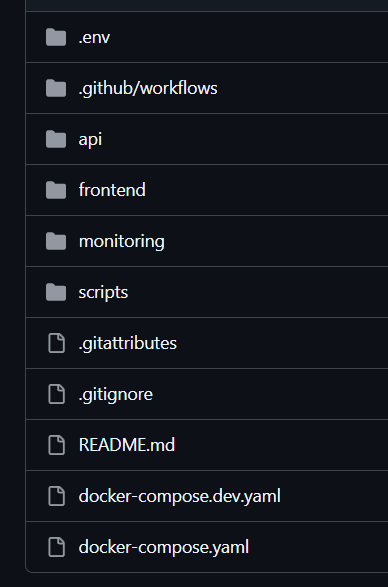
\includegraphics[height=0.9\textheight,keepaspectratio]{images/devops/struktura-projektu.png} 
    \caption*{Źródło: Opracowanie własne}
    \label{img:struktura-projektu}
\end{figure}
\subsubsection{Praca w repozytorium}
\par
Zespół przyjął uproszczoną metodologię GitFlow.
Oznacza to że każda zmiana jest tworzona na nowej gałęzi, następnie gałąź jest integrowana z gałęzią "dev".
Na koniec \gls{sprint}u zmiany z gałęzi "dev" zostają wrzucanie na gałąź główną - "main".
\par
W momencie wypracowania wersji spełniającej wymagania zespołu tworzony jest tag z konkretną wersją.
\begin{figure}[H]
    \centering
    \caption{Przykładowa pierwsza wersja systemu przygotowana na prezentację wstępną}
    
\includegraphics[width=1.0\textwidth]{images/devops/przykladowa-pierwsza-wersja-projektu.png} 
    \caption*{Źródło: Opracowanie własne}
    \label{img:przykladowa-pierwsza-wersja-projektu}
\end{figure}
\subsubsection{Integrowanie zmian}
\par
Integracje zmian wykonuje za pomocą PR(\gls{Pull Request}).
Zablokowane zostało bezpośrednie wrzucanie zmian na gałąź główną albo "dev".
Wymagania aby \glslink{Pull Request}{PR} został zaakceptowany: 
\begin{itemize}
    \item co najmniej jeden członek zespołu musi zaakceptować zmiany
    \item testy (status checki) muszą zakończyć się sukcesem
\end{itemize}
\begin{figure}[H]
    \centering
    \caption{Przykładowy \gls{Pull Request}}
    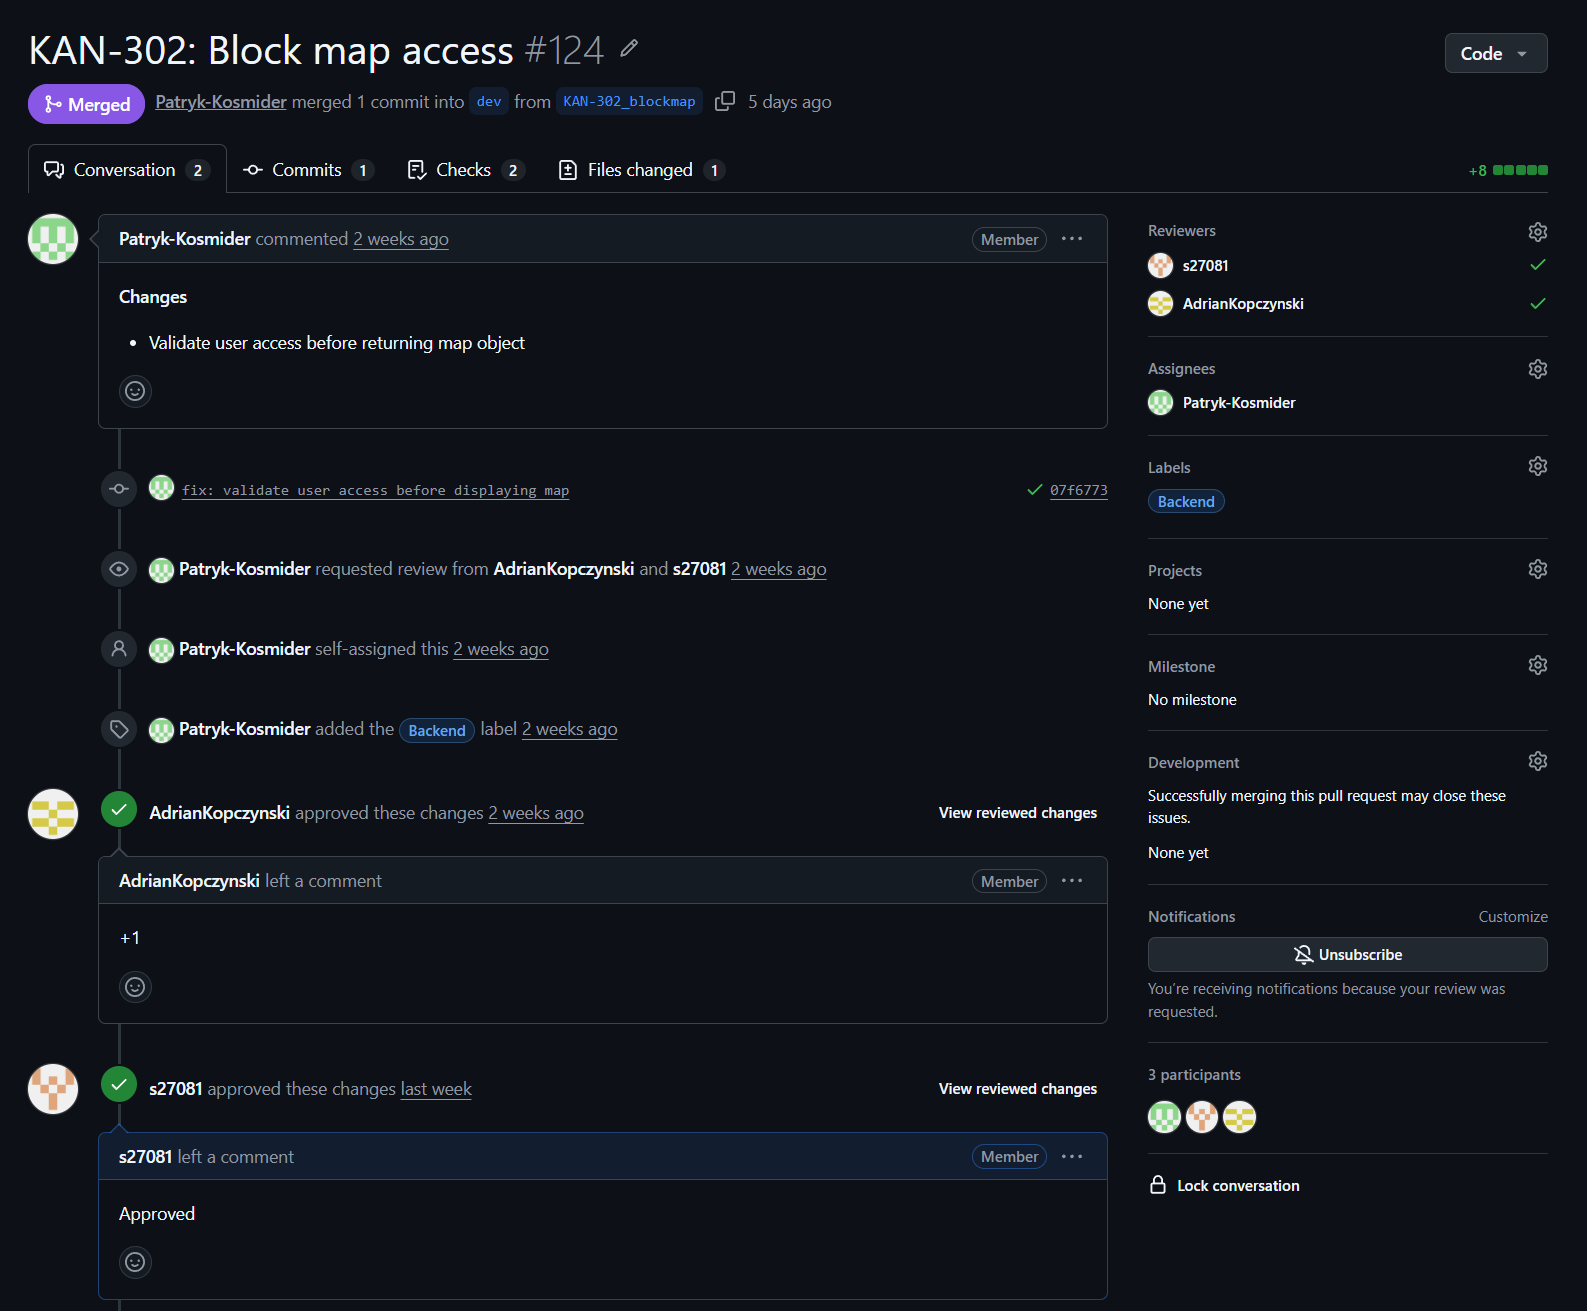
\includegraphics[width=1.0\textwidth]{images/devops/przykladowy-PR.png} 
    \caption*{Źródło: Opracowanie własne}
    \label{img:przykladowy-PR}
\end{figure}

\subsubsection{GitHub Actions}
\par
Projekt posiada kilka \gls{workflow}'ów:
\subsubsection{Testowanie}
\par
Aplikacja przed \glslink{merge}{zmergowaniem} musi przejść testy.
Testy są uruchamiane automatycznie za pośrednictwem akcji w momencie stworzenia \glslink{Pull Request}{PR}.
System automatycznie wykrywa jaka część systemu został zmieniona i na tej podstawie decyduje jakie testy uruchomić.
\par
Dodatkową funkcjonalnością było dodanie opcji “test on comment”, która umożliwiała uruchamianie testów przez wstawienie komentarza w \glslink{Pull Request}{PR}: "/test" i po spacji nazwa aplikacji do przetestowania np. "/test api"
\begin{figure}[H]
    \centering
    \caption{Uruchamianie testów używając komentarza}
    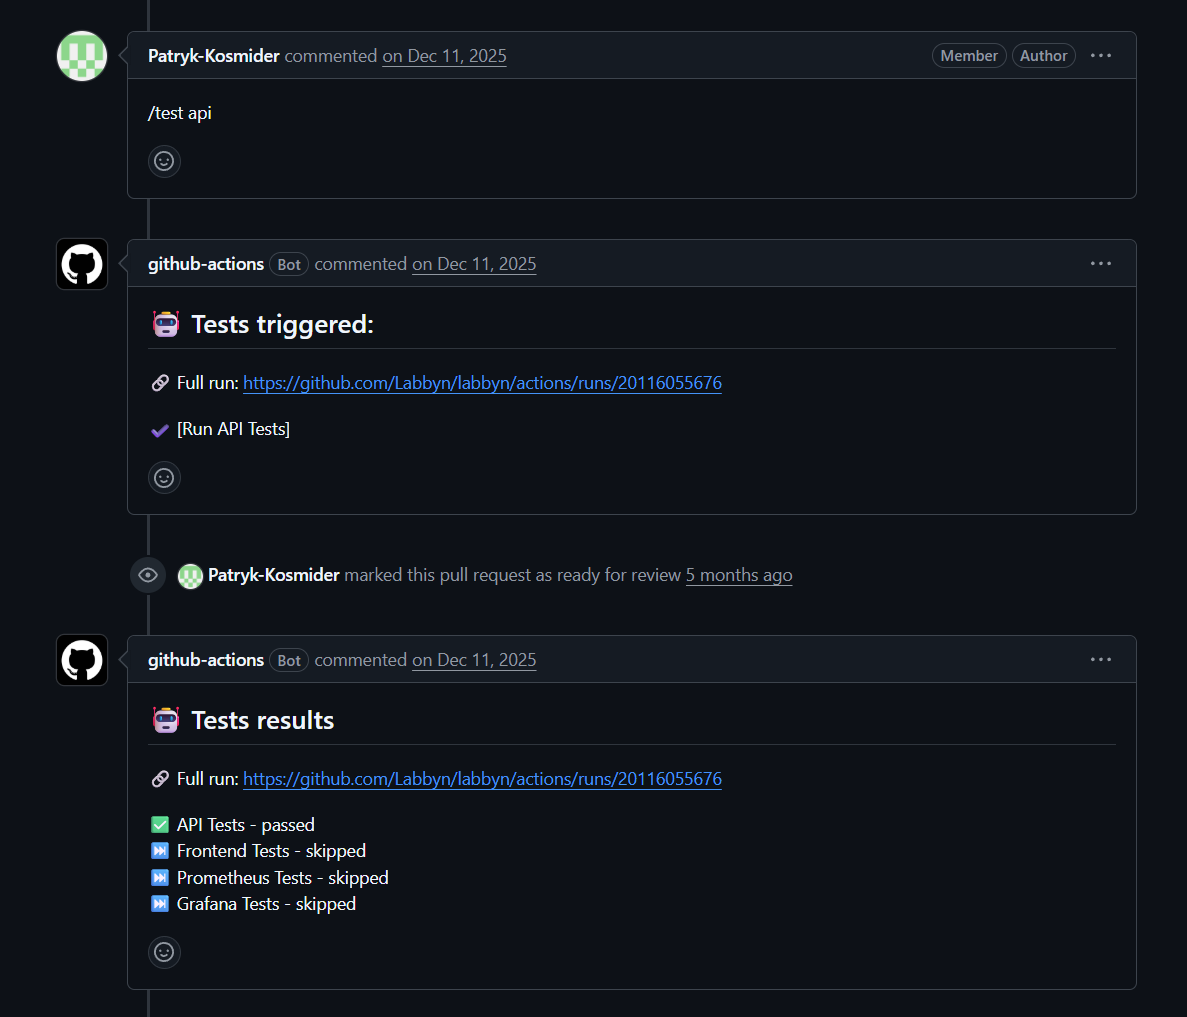
\includegraphics[width=1.0\textwidth]{images/devops/uruchamianie-testow-przez-komentarz.png} 
    \caption*{Źródło: Opracowanie własne}
    \label{img:uruchamianie-testow-przez-komentarz}
\end{figure}
\begin{figure}[H]
    \centering
    \caption{Przykładowe wywołanie testów \gls{API}}
    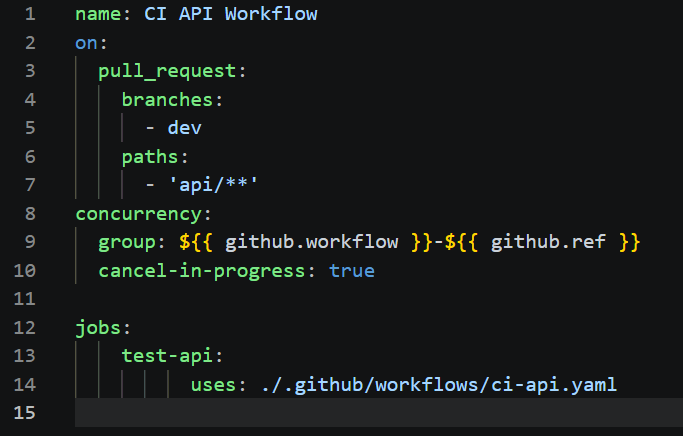
\includegraphics[width=1.0\textwidth]{images/devops/przykladowe-wywolanie-testow-api.png} 
    \caption*{Źródło: Opracowanie własne}
    \label{img:przykladowe-wywolanie-testow-api}
\end{figure}
\subsubsection{Budowanie \gls{kontener}ów i wrzucanie ich na DockerHub}
\par
Gdy główna gałąź otrzyma nowe zmiany system automatycznie buduje \gls{kontener}y aplikacji tworzone przez nas (frontend i \gls{Backend}) i wrzuca je na dedykowane \gls{repozytorium} na DockerHub.
\subsubsection{Lint}
W momencie stworzenia \glslink{Pull Request}{PR} “linter” sprawdza czy kod jest zgodny z wcześniej przygotowanymi wytycznymi dotyczącymi formatowania kodu.
Ta akcja tylko informuje o błędzie, w zespole uzgodniono aby ta akcja nie wykonywała się automatycznie.
\begin{figure}[H]
    \centering
    \caption{Przykładowy błąd z lintera}
    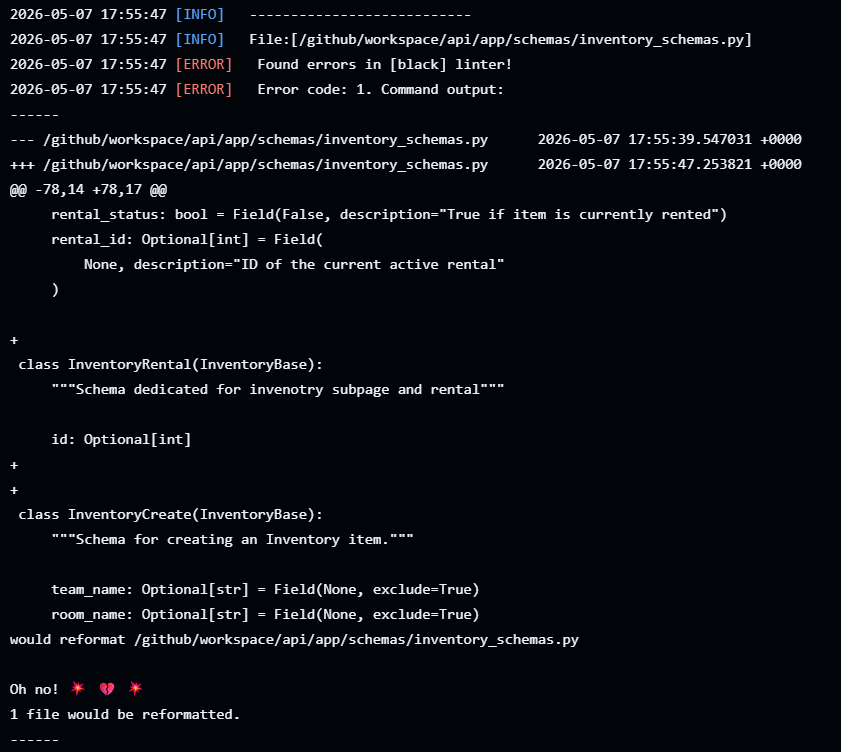
\includegraphics[width=1.0\textwidth]{images/devops/przykladowy-error-linter.png} 
    \caption*{Źródło: Opracowanie własne}
    \label{img:przykladowy-error-linter}
\end{figure}
\subsubsection{Release}
\par
\Gls{workflow} tworzący nowy tag dla nowej wersji aplikacji.
\subsubsection{Dodatki}
\par
\Gls{repozytorium} zostało zintegrowane z systemem Jira.
Dzięki temu na tablicy z zadaniami jest widoczne odwołanie do konkretnej gałęzi na \gls{GitHub}ie.
Pozwala to na lepsze śledzenie postępów zespołu.
\begin{figure}[H]
    \centering
    \caption{Przykładowe zadanie z widocznym statusem implementacji}
    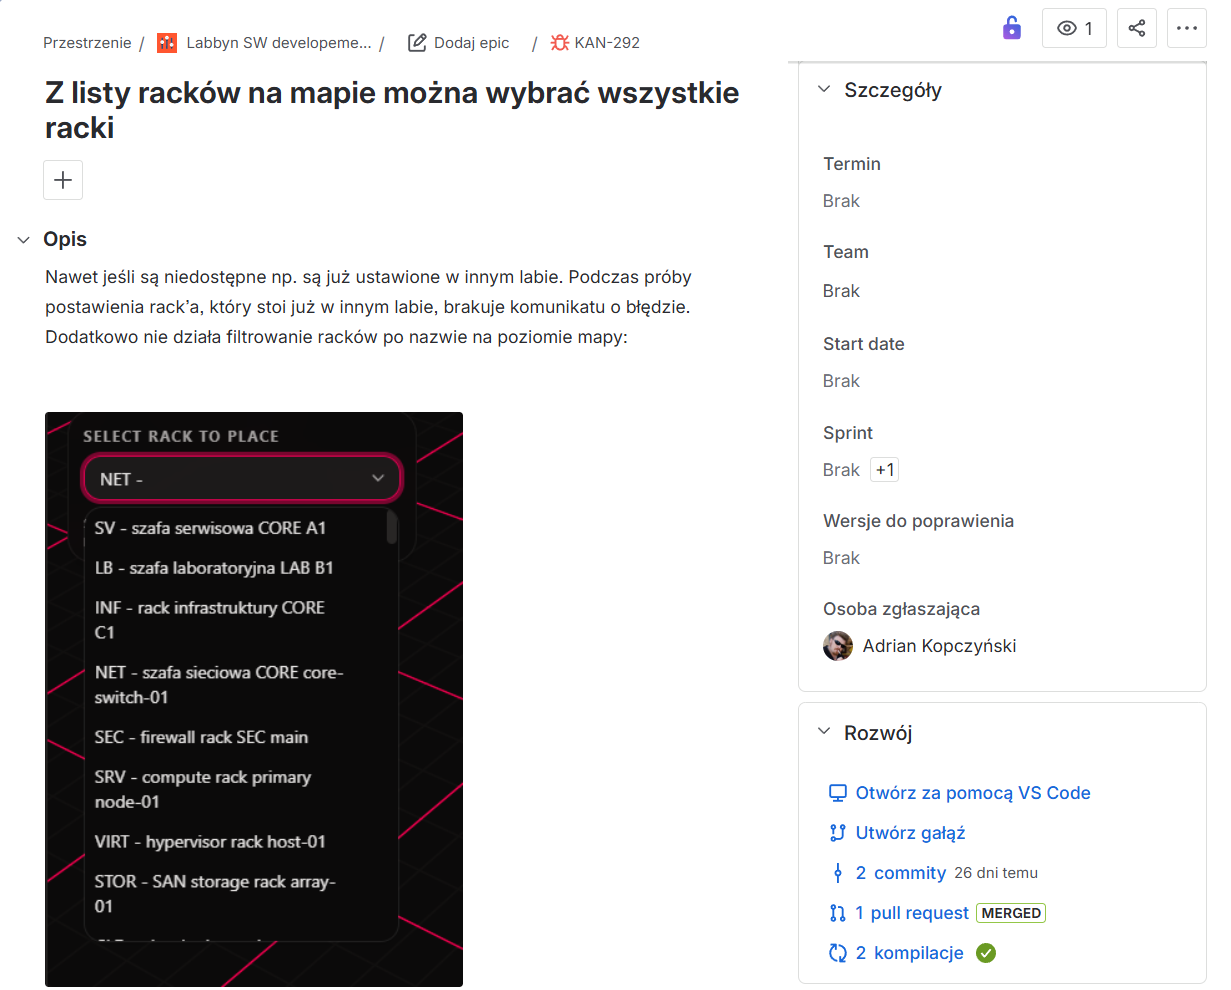
\includegraphics[width=1.0\textwidth]{images/devops/przykladowe-zadanie-z-pokazany-statusem.png} 
    \caption*{Źródło: Opracowanie własne}
    \label{img:przykladowe-zadanie-z-pokazany-statusem}
\end{figure}

\subsection{Repozytorium latex-enironment}
\par
Repozytorium przeznaczone do przechowywania wszystkich plików potrzebnych do niniejszego dokumentu.
\subsubsection{Struktura porjektu}
\par
Repozytorium zawiera pliki .tex, .cls, .bib potrzebne do budowania dokumentów oraz folder images, w którym znajdują się zrzuty ekranu potrzebne do pracy inżynierskiej.
\subsubsection{Praca w repozytorium}
\par
Ze względu na mniejszą intensywność wprowadzania zmian zespół przyjął następująca strategię: każda zmiana jest tworzona na nowej gałęzi, następnie gałąź jest integrowana z gałęzią główną. 
\subsubsection{Integrowanie zmian}
Podobnie jak przy \gls{repozytorium} "Labbyn" zmiany integrowane są za pomocą \glslink{Pull Request}{PR}.
Wymagania wyglądają następująco:
\begin{itemize}
    \item każdy członek zespołu musi zaakceptować zmiany
\end{itemize}
Dzięki takiemu podejściu każdy członek zespołu zapozna się z nową część dokumentu, a w razie wątpliwości może zażądać zmian lub zaproponować inne rozwiązanie.

\subsection{Architektura aplikacji}
\par
Aplikacja oparta jest na osobnych, skonteneryzowanych serwisach.
Ze względu na skalę projektu oraz dostępny czas usługi zostały podzielone w sposób następujący:
\begin{itemize}
    \item \textbf{api (backend)}  - aplikacja \gls{FastAPI} -  pośrednicząca między użytkownikiem, a bazą danych.
    \item \textbf{frontend} - aplikacja \gls{React}'a - odpowiedzialna za prezentację strony i przyjmowanie zapytań użytkownika.
    \item \textbf{db} - baza danych \gls{PostgreSQL}.
    \item \textbf{redis} - baza do przetrzymywania niedawno wykonanych zapytań w celu przechowania ich do przyszłego użycia w aplikacji.
    \item \textbf{adminer} - lekki \gls{kontener} umożliwiający połączenie się do bazy danych przez przeglądarkę. Graficzne przedstawia tabele i umożliwa wykonywanie operacji na bazie.
    \item \textbf{monitoring} - aplikacja \gls{Prometheus}a - odpowiedzialny za komunikację z agentami na hostach i przetwarzanie przekazanych metryk.
    \item \textbf{logging} - \gls{kontener} \glslink{Grafana}{Grafany} - umożliwiający pokazanie danych zebranych przez \gls{Prometheus}a w postaci wykresów i tabel informacyjnych.
\end{itemize}
\subsubsection{Obsługa aplikacji}
\par
Zarządzanie \gls{kontener}ami oddane jest w ręce narzędzia \gls{Docker Compose}.
Na podstawie plików docker-compose.yaml i docker-compose-dev.yaml budowana jest aplikacja.
Dzięki temu użytkownik nie marnuje czasu na ręczne konfigurowanie każdej aplikacji po kolei ręcznie.
Budowanie wykonuje się za pomocą jednej komendy.
\begin{figure}[H]
    \centering
    \caption{Konfiguracja \gls{Docker Compose}}
    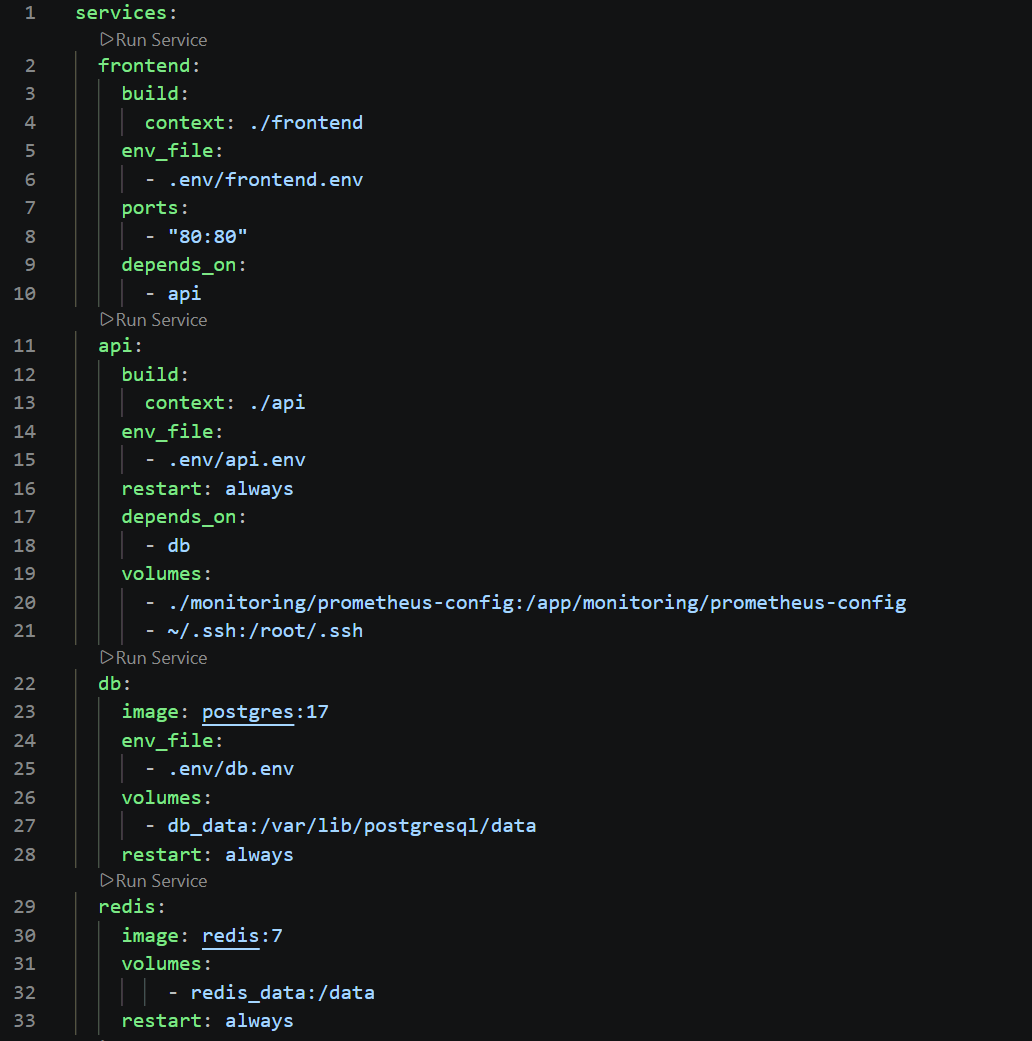
\includegraphics[width=1.0\textwidth]{images/devops/konfiguracja-docker-compose.png} 
    \caption*{Źródło: Opracowanie własne}
    \label{img:konfiguracja-docker-compose}
\end{figure}
\par
Ze względu na to że aplikacje mogą zachowywać się trochę inaczej w wersji deweloperskiej, przygotowany jest docker-compose-dev.yaml.
Nadpisuje on część konfiguracji z docker-compose.yaml dzięki czemu nasze aplikacje mogą działać w innym trybie, budować się z innego Docekerfile, na innym porcie albo korzystać z innych plików środowiskowych bez konieczności duplikowania kodu tworząc całą nową konfigurację od zera.
\par
Wersja deweloperska aplikacji jest mniej restrykcyjna. Umożliwia bezpośrednie łączenie się do skonteneryzowanych aplikacji, każdy port jest otwarty.
Ułatwia to debugowanie problemów, szybkie zmiany oraz testowanie nowych rozwiązań od razu po wprowadzeniu dzięki metodzie \gls{hot-reload}.
\begin{figure}[H]
    \centering
    \caption{''Nakładka'' na głowny plik \gls{Docker}a, który edytuje odpowiednie pola}
    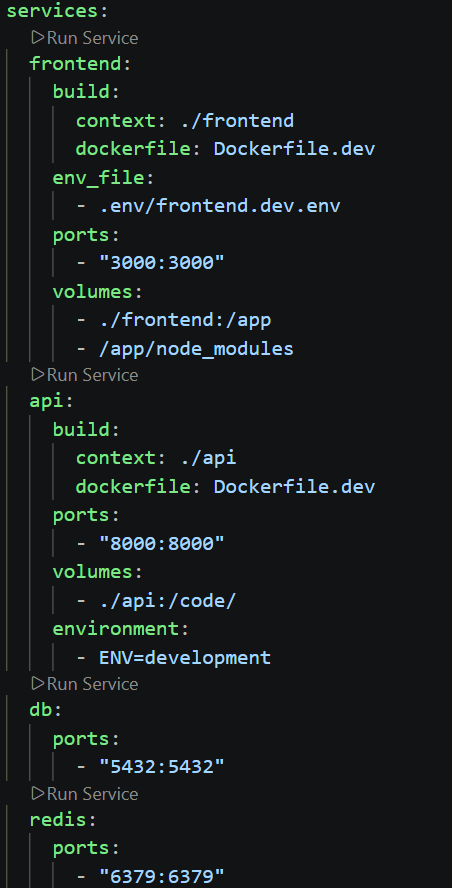
\includegraphics[width=0.75\textwidth]{images/devops/nakladka-na-glowny-plik-dockerowy.png} 
    \caption*{Źródło: Opracowanie własne}
    \label{img:nakladka-na-glowny-plik-dockerowy}
\end{figure}
\par
Dodatkowo nasz \gls{Docker Compose} został opakowany w \gls{skrypt} Bash'owy ułatwiający zarządzanie stanem całej aplikacji:
\begin{figure}[H]
    \centering
    \caption{Skrypt do zarządzania aplikacją}
    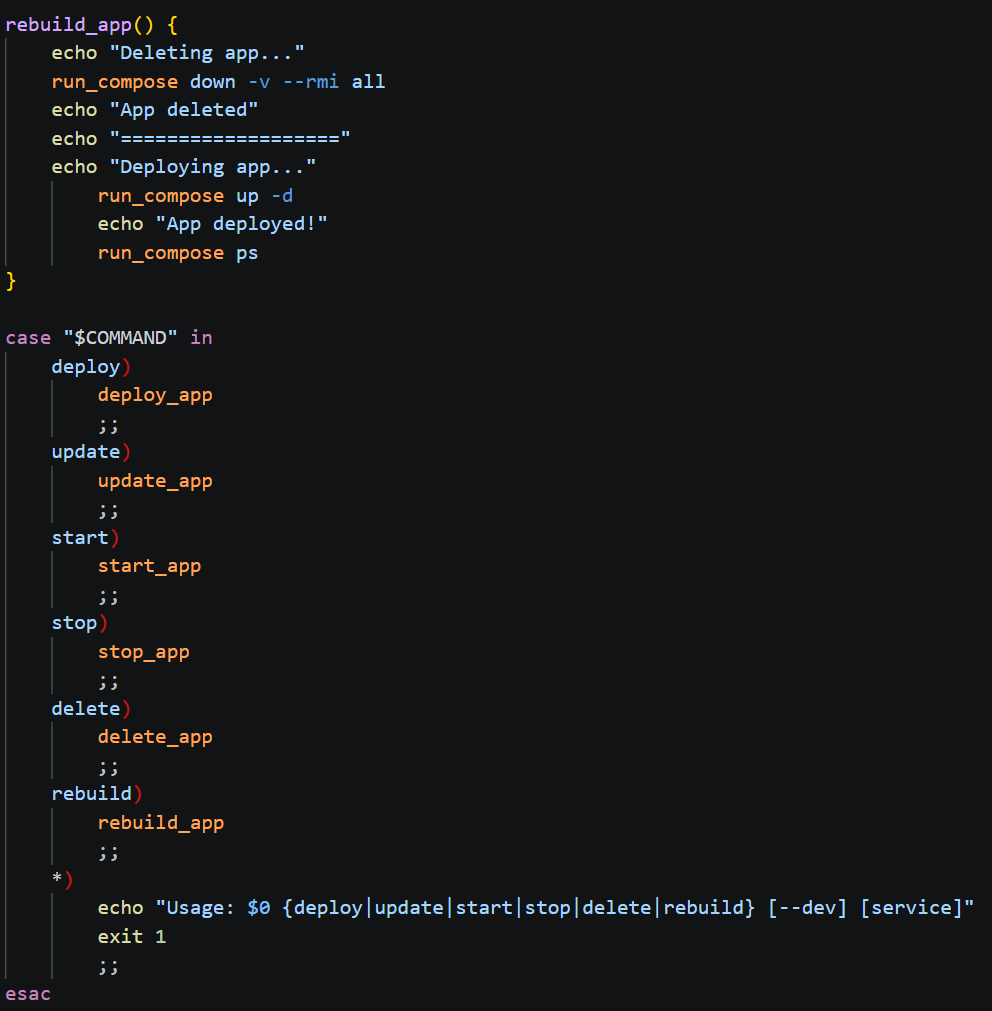
\includegraphics[width=1.0\textwidth]{images/devops/skrypt-do-zarzadzania-aplikacja.png} 
    \caption*{Źródło: Opracowanie własne}
    \label{img:skrypt-do-zarzadzania-aplikacja}
\end{figure}
\subsubsection{Kontenery}
\par
W naszym projekcie budowane są dwa \gls{kontener}y - "backend" i "frontend".
Pozostałe to wykorzystane technologie \gls{open-source} opakowane w \gls{kontener}.
\par
Do zbudowania \gls{kontener}a potrzebny jest plik Dockerfile, który służy do stworzenia obrazu \gls{kontener}a - on definiuje co znajdzie się w \gls{kontener}ze i jak będzie skonfigurowany.
\par
W budowie \gls{kontener}a najważniejsze jest odpowiednie ułożenie instrukcji.
Spowodowane jest to tym, że przy budowie obrazu \gls{Docker}owego posiłkuje się już stworzonymi warstwami, jeśli któraś warstwa (każda instrukcja to jedna warstwa) jest inna to reszta musi zostać ponownie zbudowana co wydłuża całkowity czas budowania obrazu.
\par
Dodatkowym zabiegiem, który warto wykonać jest Multi-Stage building.
Umożliwia on stworzenie jednego \gls{kontener}a - buildera, na którym pobierane są wszystkie zależności wymagane do zbudowania aplikacji.
Obraz jest budowany, a następnie pliki zbudowanej aplikacji zostaną skopiowane na nowy \gls{kontener} - production.
Dzięki temu możemy zmniejszyć wielkość obrazu przez brak zależności wymaganych do budowy oraz nowy obraz nie będzie posiadał różnych artefaktów stworzonych w trakcie budowania aplikacji, chyba że my sprecyzujemy aby je skopiować
\begin{figure}[H]
    \centering
    \caption{Dockerfile aplikacji \gls{Frontend}}
    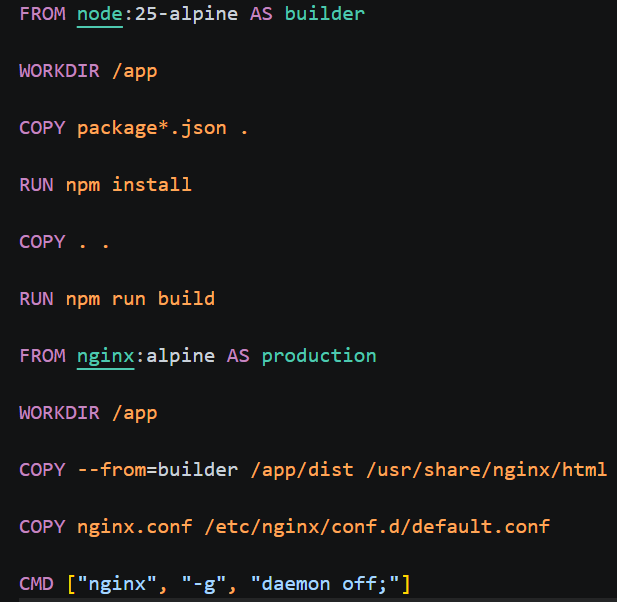
\includegraphics[width=1.0\textwidth]{images/devops/dockerfile-aplikacji-frontned.png} 
    \caption*{Źródło: Opracowanie własne}
    \label{img:dockerfile-aplikacji-frontned}
\end{figure}
\subsubsection{Maszyny wirtualne}
\par
Z racji na ograniczenia budżetowe oraz infrastrukturalne, testowanie platform pod względem zgodności z naszą aplikacją zgodnie z wymaganiami odbyło się z wykorzystaniem maszyn wirtualnych.
Do tego wykorzystane zostało narzędzie \gls{Vagrant}.
\par
\gls{Vagrant} umożliwia nam tworzenie maszyn wirtualnych wykorzystując podejście \gls{IaC}, co pozwala zdefiniować nam konfiguracje maszyn wirtualnych w pliku Vagrantfile.
Na podstawie tego, \gls{Vagrant} automatycznie instaluje odpowiedni obraz, podpina zasoby oraz konfiguruje konta.
\par
Na potrzeby naszej pracy inżynierskiej powstał plik tworzący dwie maszyny wirtualne do testów.
Celem było ułatwienie testowania, jednocześnie nie obciążając nadmiernie platform deweloperskich członków zespołu.
\begin{figure}[H]
    \centering
    \caption{Konfiguracja dwóch wirtualnych maszyn}
    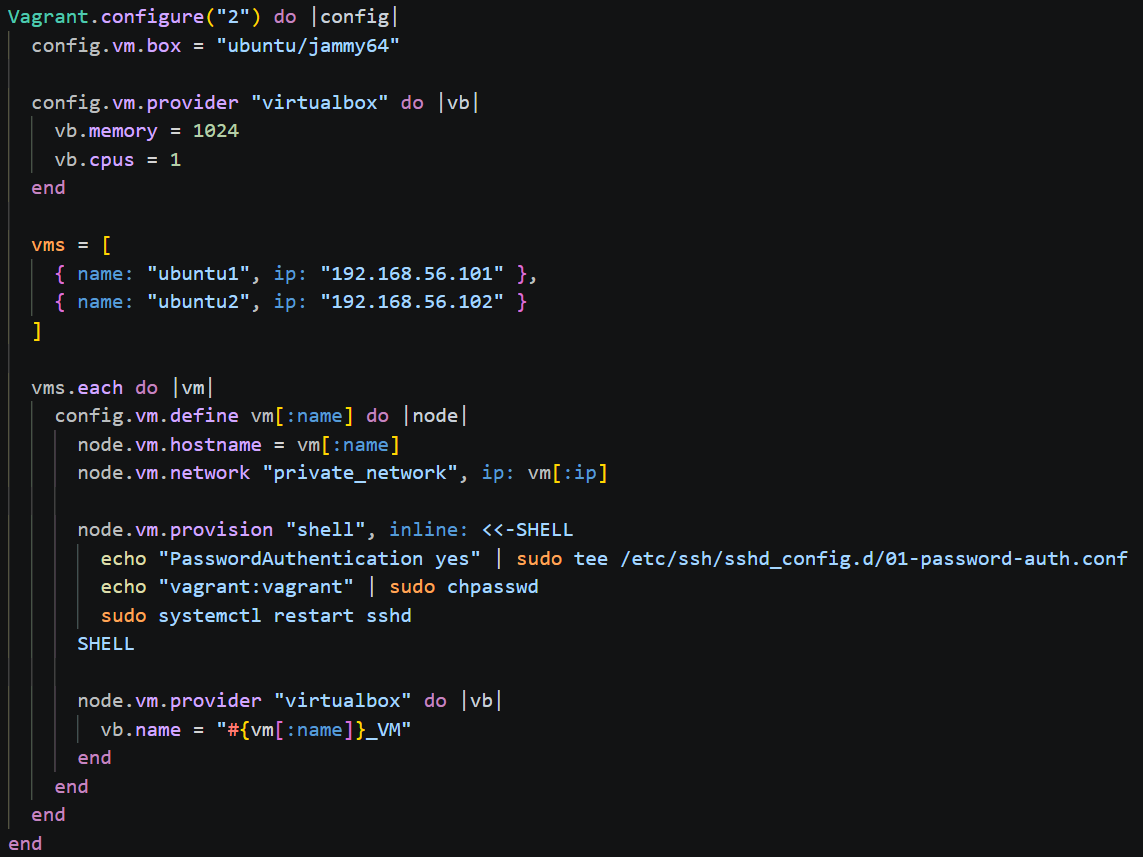
\includegraphics[width=1.0\textwidth]{images/devops/konfiguracja-dwoch-maszyn-wirtualnych.png} 
    \caption*{Źródło: Opracowanie własne}
    \label{img:konfiguracja-dwoch-maszyn-wirtualnych}
\end{figure}

